\documentclass[nooutcomes, handout]{ximera}
%% handout
%% space
%% newpage
%% numbers
%% nooutcomes
\usepackage{booktabs}
%I added the commands here so that I would't have to keep looking them up
%\newcommand{\RR}{\mathbb R}
%\renewcommand{\d}{\,d}
%\newcommand{\dd}[2][]{\frac{d #1}{d #2}}
%\renewcommand{\l}{\ell}
%\everymath{\displaystyle}
%\newcommand{\dfn}{\textbf}
%\newcommand{\eval}[1]{\bigg[ #1 \bigg]}

\usepackage{fullpage}
\newcommand{\RR}{\mathbb R}
\renewcommand{\d}{\,d}
\newcommand{\dd}[2][]{\frac{d #1}{d #2}}
\renewcommand{\l}{\ell}
\newcommand{\ddx}{\frac{d}{dx}}
\newcommand{\dfn}{\textbf}
\newcommand{\eval}[1]{\bigg[ #1 \bigg]}

\usepackage{multicol}

\renewenvironment{freeResponse}{
\ifhandout\setbox0\vbox\bgroup\else
\begin{trivlist}\item[\hskip \labelsep\bfseries Solution:\hspace{2ex}]
\fi}
{\ifhandout\egroup\else
\end{trivlist}
\fi} %% we can turn off input when making a master document

\title{Section 3.4 The Product and Quotient Rules}  

\begin{document}
\begin{abstract}		\end{abstract}
\maketitle

%Problem1
\begin{problem}
 Differentiate the function $f$ defined by $f(x) = 1/x^8$ in two different ways.
  \begin{freeResponse}
    Applying the quotient rule:
    \begin{align*}
      f'(x) &= \frac{(1)' \cdot x^8 - (1 \cdot (x^8)')}{(x^8)^2} \\
            &= \frac{(0 \cdot x^8) - (1 \cdot 8x^7)}{x^{16}} \\
            &= \frac{-8x^7}{x^{16}}\\
            &= \frac{-8}{x^9}. 
    \end{align*}

  Applying the power rule:
  \begin{align*}
    f(x) &= \frac{1}{x^8} = x^{-8}\\
    &\implies f'(x) = (x^{-8})'\\
    &= -8\cdot x^{-8 -1}\\
    &= -8x^{-9}
  \end{align*}
  \end{freeResponse}
\end{problem}
	
%problem 2			
\begin{problem}
Suppose that $f(5) = 7$, $f'(5) = 8$, $g(5) = 3$, and $g'(5) = -4$.  Find:

	\begin{enumerate}

	\item  $(fg)'(5)$.
		\begin{freeResponse}
		\begin{align*}
		(fg)'(5) &= (f'(5) \cdot g(5)) + (f(5) \cdot g'(5))  \\
		&= (8)(3) + (7)(-4)  \\
		&= 24 - 28 = -4.
		\end{align*}
		\end{freeResponse}
		
		

	\item $\left[ \ddx \left( \frac{f}{g} \right) \right]$
		\begin{freeResponse}
		\begin{align*}
		\left[ \ddx \left( \frac{f}{g} \right) \right] (5) &= \frac{(g(5) \cdot \left[ \ddx f \right] (5)) - (f(5) \cdot \left[ \ddx g \right](5))}{(g(5))^2}  \\
		&= \frac{(3)(8) - (7)(-4)}{3^2}  \\
		&= \frac{24 + 28}{9} = \frac{52}{9}.
		\end{align*}
		\end{freeResponse}
		
		
	\item $ \left( \frac{g}{f} \right)' (5)$
		\begin{freeResponse}
		\begin{align*}
		\left( \frac{g}{f} \right)' (5) &= \frac{(f(5) \cdot g'(5)) - (g(5) \cdot f'(5))}{(f(5))^2}  \\
		&= \frac{(7)(-4) - (3)(8)}{7^2}  \\
		&= \frac{-28 - 24}{49} = - \frac{52}{49}.
		\end{align*}
		\end{freeResponse}
		
	\item  $\eval{ \ddx \left( \frac{g}{x+2} \right) (x)}_{x=5}$
		\begin{freeResponse}
		\begin{align*}
		\eval{\ddx \left( \frac{g}{x+2} \right) (x)}_{x=5} &= \eval{\frac{(x+2) \cdot g'(x)) - (g(x) \cdot (x+2)'}{(x+2)^2}}_{x=5}  \\
		&= \frac{(x+2)(-4) - (3)(1)}{(5+2)^2}  \\
		&= \frac{(7)(-4) - (3)(1)}{7^2}  \\
		&= \frac{-28 - 3}{49} = - \frac{31}{49}
		\end{align*}
		\end{freeResponse}



	\item $\eval{ \ddx \left( \frac{xf(x)}{g(x)} \right) (x)}_{x=5}$
		\begin{freeResponse}
		\begin{align*}
		\eval{\ddx \left( \frac{xf(x)}{g(x)} \right) (x)}_{x=5} &= \eval{\frac{(((xf(x))' \cdot g(x)) - (g'(x) \cdot (xf(x)))}{(g(x))^2}}_{x=2}  \\
		&= \eval{\frac{\left( (x)' \cdot f(x)+x \cdot f'(x) \right) \cdot g(x)) - (g'(x) \cdot (xf(x))}{(g(x))^2}}_{x=5}  \\
		&= \frac{(1 \cdot 7+ 5 \cdot 8)(3) - (-4)(5)(7)}{(3)^2}  \\
		&= \frac{50 - 140}{9}  \\
		&= \frac{-90}{9} = - 10
		\end{align*}
		\end{freeResponse}

	\end{enumerate}
		
\end{problem}




%problem 3	
\begin{problem}
  Use the given information to find the equation of the tangent line.
  \begin{enumerate}
    \item
      Given $g(x) = x^3 f(x)$, $f(2) = 4$, and $f'(2) = 7$, find the equation of the tangent line to the graph of $g$ at $x = 2$.
      \begin{freeResponse}
        Slope of tangent line to the graph of $g$ at the point where $x = 2$:
        \begin{align*}
          g'(x) &= 3x^2 f(x) + x^3 f'(x)\\
          &\implies g'(2) = 12(4) + 8(7) = 48 + 56 = 104.
        \end{align*}

        Point on tangent line where $x=2$: $(2, g(2)) = (2, 8f(2)) = (2, 32)$.

        Equation of tangent line:
        \begin{align*}
          y-32 &= 104(x-2)\\
          &\implies y = 104x - 176.
        \end{align*}
      \end{freeResponse}


    \item
      Given $h(z) = \frac{z s(z)}{z-3}$, $s(2) = 4$, and $s'(2) = 7$, find the equation of the tangent line to the graph of $h$ at $z = 2$.
      \begin{freeResponse}
        Slope of tangent line to the graph of $h$ at the point where $z = 2$:
        \begin{align*}
          h'(z) &= \frac{ (z-3)(z s(z))' - z s(z)(z-3)'}{(z-3)^2}  \\
		&= \frac{(z-3)(s(z) + z s'(z)) - z s(z)(1)}{(z-3)^2} \\
                &\implies h'(2) = \frac{(2-3)(s(2) + 2 s'(2)) - 2s(2)}{(2-3)^2} = -26.
        \end{align*}

        Point on tangent line where $z=2$: $(2, h(2)) = (2, \frac{2s(2)}{2-3}) = (2, -8)$.

        Equation of tangent line to the graph of $h$ at the point where $z=2$:
        \begin{align*}
          y-(-8) &= -26(z-2) \\
          &\implies y = -26z + 44.
        \end{align*}
      \end{freeResponse}


    \item
      Given
      \begin{center}
        \begin{tabular}{cccccc}
       \toprule
          $x$ & 1 & 2 & 3 & 4 & 5\\
     \midrule
          $f(x)$ & 5 & 3 & 0 &$-4$ & 3\\
          $f'(x)$ & $-3$ & $-5$ & $-2$ & 6& $-4$\\
          $g(x)$ & 6 &9&$-8$&13&15\\
          $g'(x)$ & 8 & 5 & $-10$ &7& 6\\
  	\bottomrule
        \end{tabular}
      \end{center}
      find the equation of the tangent line of 
      \[
        \frac{f(x)}{e^xg(x)}
      \]
      at $x = 2$.
      \begin{freeResponse}
        Slope of tangent line to the graph of $ \frac{f(x)}{e^xg(x)} $ at the point where $x=2$:
        \begin{align*}
          \left( \frac{f(x)}{e^x g(x)} \right)'
          &= \frac{e^x g(x) f'(x) - f(x)(e^x g(x) + e^x g'(x))}{(e^x g(x))^2}.  \\
          &\implies \frac{d}{dx}\left(\frac{f(x)}{e^x g(x)}\right) \bigg|_{x=2}
          = \frac{e^2 g(2) f'(2) - f(2)(e^2 g(2) + e^2 g'(2))}{(e^2 g(2))^2}  \\
		&= \frac{e^2 (9)(-5) - (3)(9e^2 + 5e^2)}{(9e^2)^2}  \\
		&= \frac{-45e^2 -42e^2}{81e^4}  \\
		&= \frac{-87e^2}{81e^4}\\
                  &= \frac{-87}{81e^2}
        \end{align*}

        Point on tangent line where $x=2$: $(2, f(2)/(e^2g(2))) = (2, 3/(9e^2)) = (2, 1/(3e^2))$.

        Equation of tangent line where $x=2$:
        \begin{align*}
          y - \frac{1}{3e^2} &= \frac{-87}{81e^2}(x - 2)\\
                             &\implies y = \frac{-87}{81e^2}x  + \frac{67}{27e^2}.
        \end{align*}
      \end{freeResponse}
   \end{enumerate}
\end{problem}

%problem 4
\begin{problem}
Differentiate the following functions:

	\begin{enumerate}
	
	%part a
	\item  Given $f(x) = (x^2 + 4x - 7) e^{-2x}$, show $f'(x)=(-2x^2 - 6x + 18)e^{-2x}$.
			\begin{freeResponse}
			\begin{align*}
			f'(x) &= \left( \ddx(x^2 + 4x - 7) \cdot e^{-2x} \right) + \left((x^2 + 4x - 7) \cdot \ddx(e^{-2x}) \right)  \\
			&= ((2x+4)(e^{-2x}) + (x^2 + 4x - 7)(-2e^{-2x})  \\
			&= (2x + 4 - 2x^2 - 8x + 14)e^{-2x}  \\
			&= (-2x^2 - 6x + 18)e^{-2x}.
			\end{align*}
			\end{freeResponse}
			
			
			
	%part b
	\item  Given $g(x) = \frac{x^2 + 4x - 7}{e^{-2x}}$, show $g'(x)=\frac{2x^2 + 10x - 10}{e^{-2x}}$
			\begin{freeResponse}
			\begin{align*}
			g'(x) &= \frac{\left( e^{-2x} \cdot \ddx(x^2 + 4x - 7) \right) - \left( (x^2 + 4x - 7) \cdot \ddx(e^{-2x}) \right)}{(e^{-2x})^2}  \\
			&= \frac{((e^{-2x}) \cdot (2x+4)) - ((x^2 + 4x - 7) \cdot (-2e^{-2x}))}{e^{-4x}}  \\
			&= \frac{(2x + 4 + 2x^2 + 8x - 14)e^{-2x}}{e^{-4x}}  \\
			&= \frac{2x^2 + 10x - 10}{e^{-2x}}.
			\end{align*}
			\end{freeResponse}
			
			
			
			
	\end{enumerate}		
\end{problem}
	
%problem5
\begin{problem}
	The graph of a function $g$ is given below.  Using the graph, estimate the derivative at the given point: \\
	$\ddx \left({\frac{xg(x)}{x+3}}\right)\ \text{at}\ x=1$

   \begin{image}
     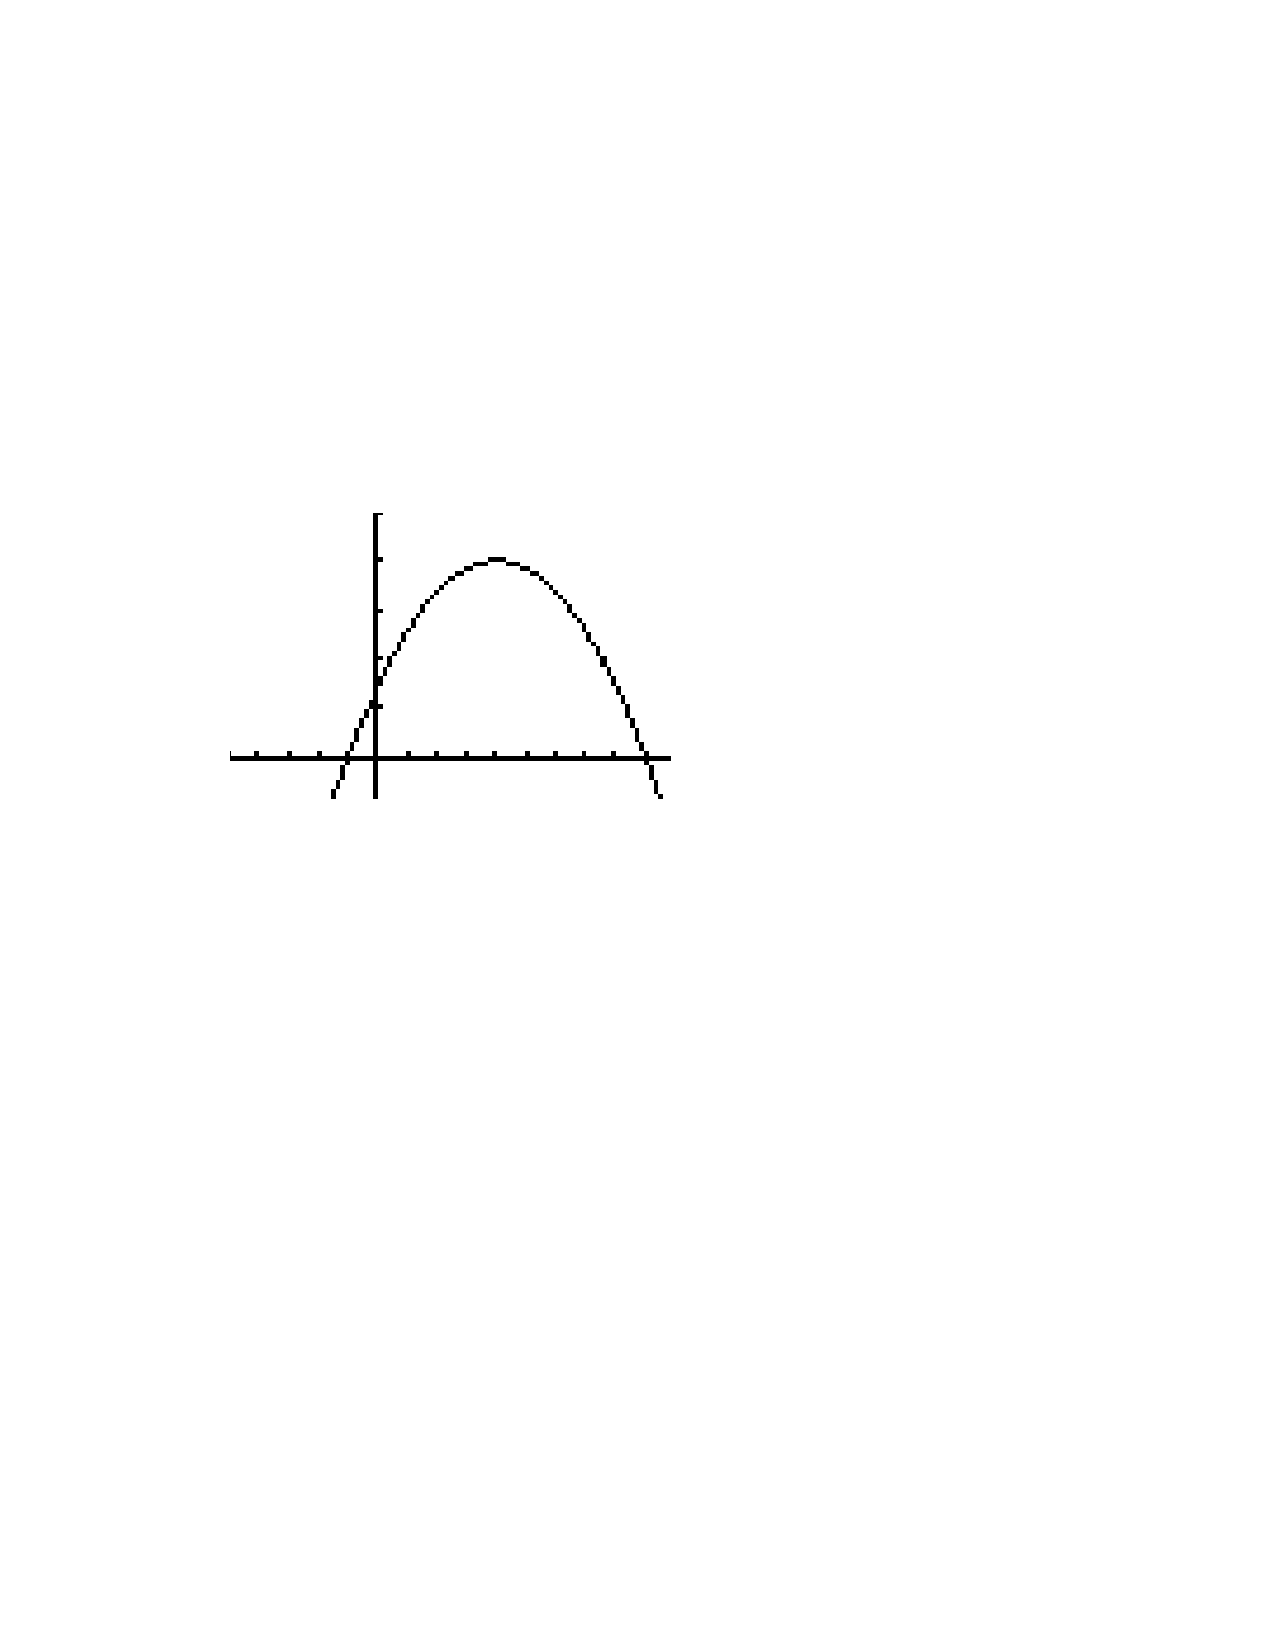
\includegraphics[scale = 0.5]{Figure1.png}
   \end{image}

	\begin{freeResponse}
		From the graph it appears that $g(1)=2$.  We can draw the line tangent to the curve $y=g(x)$ at the point $(1,g(1))$
  		 \begin{image}
    			 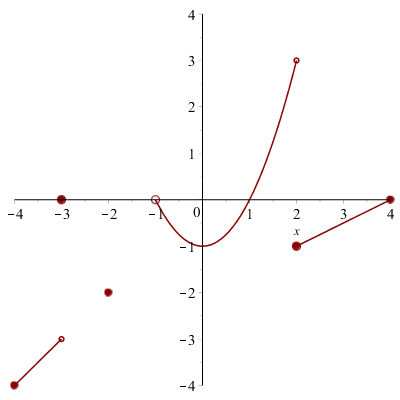
\includegraphics[scale = 0.5]{Figure2.png}
 		  \end{image}
		
		Since $g'(1)$ is the slope of the line tangent to the curve $y=g(x)$ at the point $(1,g(1))$, we can estimate its slope of the line.  It seems that when $x$ grows by any $\Delta x$, $y$ also grows by the same amount.  So the slope $=g'(1) \approx 1$.  Therefore,

	\begin{align*}
	\eval{ \ddx \left( \frac{xg(x)}{x+2}\right)}_{x=1}&= \eval{\frac{(g(x)+xg'(x))(x+3)-xg(x)}{(x+3)^2}}_{x=1}\\
	&=\frac{(g(1)+1g'(1))(1+3)-(1)g(1)}{(1+3)^2} \\
	& \approx \frac{(2+1(1))(4)-1(2)}{4^2}\\
	&=\frac{(2+1)(4)-2}{16}\\
	&= \frac{3(4)-2}{16}\\
	&= \frac{12-2}{16}\\
	&= \frac{10}{16}\\
	&=\frac{5}{8}
	\end{align*}



	\end{freeResponse}

\end{problem}	
	
	
			
			


\end{document}